\documentclass[journal,11pt]{IEEEtran}

\usepackage{amsmath,amssymb,amsthm}
\usepackage{booktabs}
\usepackage{graphicx}
\usepackage{url}
\usepackage[hidelinks]{hyperref}

% IEEE house style for theorem-like environments: italic head, colon, italic body
\newtheoremstyle{ieeethm}{\topsep}{\topsep}{\itshape}{0pt}{\itshape}{:}{.5em}{}
\theoremstyle{ieeethm}
\newtheorem{proposition}{Proposition}
\newtheorem{assumption}{Assumption}
\newtheoremstyle{ieeerem}{\topsep}{\topsep}{\normalfont}{0pt}{\itshape}{:}{.5em}{}
\theoremstyle{ieeerem}
\newtheorem{remark}{Remark}
% Proofs use IEEEtran's own IEEEproof environment, which sets an italic
% "Proof:" head and closes with the filled QED box of IEEE house style.

% \input inside a tabular
\makeatletter
\newcommand{\tabinput}[1]{\@@input #1 }
\makeatother

% Generated by make_numbers.py -- do not edit by hand.
\newcommand{\quadGrid}{2\times 10^{-14}}
\newcommand{\quadNodes}{4001}
\newcommand{\quadGH}{5.1}
\newcommand{\spreadKQtrNn}{0.9}
\newcommand{\spreadKQtrNt}{4.5}
\newcommand{\spreadKHalfNn}{1.0}
\newcommand{\spreadKHalfNt}{4.9}
\newcommand{\spreadKOneNn}{2.4}
\newcommand{\spreadKOneNt}{7.9}
\newcommand{\spreadKTwoNn}{12.7}
\newcommand{\spreadKTwoNt}{23.1}
\newcommand{\inspTwoLo}{85.4}
\newcommand{\inspTwoHi}{98.1}
\newcommand{\inspTwoRule}{85.1}
\newcommand{\domMaxGap}{27.1}
\newcommand{\domOverstate}{0.4}
\newcommand{\domBest}{2.3}
\newcommand{\domSmallLam}{14.3}
\newcommand{\domBigKappa}{27.1}
\newcommand{\domModerate}{5.0}
\newcommand{\marMaxRel}{54}
\newcommand{\marMaxUnits}{676}
\newcommand{\marMedMid}{11}
\newcommand{\mpSigma}{0.6}
\newcommand{\mpMean}{8}
\newcommand{\mpTrunc}{3\times 10^{-07}}
\newcommand{\mpShipOne}{29}
\newcommand{\mpInterOne}{29}
\newcommand{\mpMixedOne}{29}
\newcommand{\mpShipTwo}{29}
\newcommand{\mpInterTwo}{23}
\newcommand{\mpMixedTwo}{26}
\newcommand{\mpShipFour}{29}
\newcommand{\mpInterFour}{19}
\newcommand{\mpMixedFour}{24}
\newcommand{\mpShipEight}{29}
\newcommand{\mpInterEight}{17}
\newcommand{\mpMixedEight}{23}
\newcommand{\mpWrongCover}{93.2}
\newcommand{\mpConsCover}{99.999}
\newcommand{\capUnits}{24}
\newcommand{\capLevels}{10/12/14}
\newcommand{\capHours}{5\,424}
\newcommand{\capCrit}{2.8}
\newcommand{\capAnyCross}{5}
\newcommand{\capSustained}{3}
\newcommand{\capEndsAbove}{0}
\newcommand{\capMaxFinal}{1.89}
\newcommand{\capFinalTen}{1.01}
\newcommand{\capFinalTwelve}{1.29}
\newcommand{\capFinalFourteen}{1.61}
\newcommand{\capSd}{0.070}
\newcommand{\nSources}{4}
\newcommand{\nSuitable}{0}
\newcommand{\dsReps}{200}
\newcommand{\dsEps}{0.3}
\newcommand{\dsBound}{0.02}
\newcommand{\dsAllocOneLo}{66}
\newcommand{\dsAllocOneHi}{84}
\newcommand{\dsAllocTenLo}{94}
\newcommand{\dsAllocTenHi}{98}
\newcommand{\dsAllocTwentyLo}{99}
\newcommand{\dsSpurShipLo}{41}
\newcommand{\dsSpurShipHi}{53}
\newcommand{\dsSpurInterLo}{19}
\newcommand{\dsSpurInterHi}{46}
\newcommand{\dsSpurShipForty}{44}
\newcommand{\dsSpurInterForty}{44}
\newcommand{\dsTenFail}{159}
\newcommand{\dsTenTauRmse}{0.20}
\newcommand{\dsTenOmRmse}{0.20}
\newcommand{\dsTenCover}{99.0}
\newcommand{\dsTenCoverPTen}{98.3}
\newcommand{\dsOneFail}{40}
\newcommand{\dsOneOmBound}{72}
\newcommand{\dsFortyTauRmse}{0.08}
\newcommand{\dsFortyCover}{99.3}
\newcommand{\dsFortyCoverPTen}{98.9}
\newcommand{\dsTwentyCover}{99.1}
\newcommand{\dsTwentyCoverPTen}{98.3}
\newcommand{\dsShipOneCoverPTen}{93.6}
\newcommand{\gridPts}{5\,664}
\newcommand{\gridLam}{236}
\newcommand{\gridSig}{8}
\newcommand{\gridLamLo}{0.05}
\newcommand{\gridLamHi}{1000}
\newcommand{\gridSigLo}{0.05}
\newcommand{\gridSigHi}{1.5}
\newcommand{\svJointOne}{29}
\newcommand{\svJointTotOne}{29}
\newcommand{\svMargOne}{29}
\newcommand{\svMargTotOne}{29}
\newcommand{\svJointTwo}{17}
\newcommand{\svJointTotTwo}{34}
\newcommand{\svMargTwo}{15}
\newcommand{\svMargTotTwo}{30}
\newcommand{\svJointFour}{11}
\newcommand{\svJointTotFour}{44}
\newcommand{\svMargFour}{9}
\newcommand{\svMargTotFour}{36}
\newcommand{\svJointEight}{7}
\newcommand{\svJointTotEight}{56}
\newcommand{\svMargEight}{5}
\newcommand{\svMargTotEight}{40}
\newcommand{\svNaiveShip}{96.4}
\newcommand{\svNaiveInter}{94.9}
\newcommand{\svNaiveShipFour}{98.3}
\newcommand{\svJointShipTwo}{17}
\newcommand{\svJointInterTwo}{18}
\newcommand{\svTotJointEight}{56}
\newcommand{\svTotJointInterEight}{56}

% Generated by make_numbers_v2.py -- do not edit by hand.
\newcommand{\spLamN}{121}
\newcommand{\spLamHi}{50}
\newcommand{\spLamLo}{0.05}
\newcommand{\spSigLo}{0.1}
\newcommand{\spSigHi}{1}
\newcommand{\spPts}{3\,630}
\newcommand{\spPoisShort}{21.2}
\newcommand{\spPoisUnits}{245}
\newcommand{\spPoisEqual}{38}
\newcommand{\spKapShort}{3.2}
\newcommand{\spKapUnits}{140}
\newcommand{\spKapEqual}{18}
\newcommand{\spNbShort}{0.4}
\newcommand{\spNbUnits}{15}
\newcommand{\spNbEqual}{70}
\newcommand{\spNbOver}{25}
\newcommand{\spCfErr}{15.9}
\newcommand{\spNbShortOp}{0.35}
\newcommand{\spKapShortOp}{2.2}
\newcommand{\spPoisShortOp}{14.4}
\newcommand{\rvSaveMed}{14}
\newcommand{\rvSaveMax}{66}
\newcommand{\rvSaveEq}{2}
\newcommand{\rvMargMin}{93.1}
\newcommand{\rvExOpt}{54}
\newcommand{\rvExCom}{56}
\newcommand{\rvConsJointMin}{99.0}
\newcommand{\rvConsAggMin}{99.0}
\newcommand{\rvAvgJointMin}{98.8}
\newcommand{\rvAvgAggMin}{97.6}
\newcommand{\fedN}{100}
\newcommand{\fedSameTheta}{4\times 10^{-8}}
\newcommand{\fedSigMed}{0.002}
\newcommand{\fedBetaMax}{0.016}
\newcommand{\fedDiverge}{16}
\newcommand{\fedRounds}{464}
\newcommand{\fedFloats}{426\,880}
\newcommand{\fedOneShot}{1\,920}
\newcommand{\fedRatio}{222}
\newcommand{\dsCells}{155}
\newcommand{\dsReps}{1\,000}
\newcommand{\dsCampaigns}{155\,000}
\newcommand{\dsFailed}{0}
\newcommand{\dsTypeOneMax}{6.1}
\newcommand{\dsTypeOneMed}{2.7}
\newcommand{\dsMcseRej}{0.7}
\newcommand{\dsCiLo}{92.0}
\newcommand{\dsCiHi}{100.0}
\newcommand{\dsCiReps}{300}
\newcommand{\dsOrderOneLo}{60}
\newcommand{\dsOrderOneHi}{71}
\newcommand{\dsOrderFour}{93}
\newcommand{\dsPowOmTwentyFour}{74}
\newcommand{\dsPowOmFortyEight}{100}
\newcommand{\dsPowOmTenFour}{46}
\newcommand{\dsPredCoverTen}{99.0}
\newcommand{\dsPlugCoverFive}{98.2}
\newcommand{\dsPoisLo}{89.2}
\newcommand{\dsPoisHi}{97.6}
\newcommand{\dsPoisMThree}{84.9}
\newcommand{\dsPoisPEight}{87.9}
\newcommand{\dsPredMin}{97.7}
\newcommand{\dsPredMThree}{98.5}
\newcommand{\dsUnitsFiveMean}{135}
\newcommand{\dsUnitsFiveMed}{28}
\newcommand{\dsUnitsOracle}{27}
\newcommand{\niTrainFail}{4\,697}
\newcommand{\niWithinTrain}{2\,962}
\newcommand{\niWithinTest}{1\,735}
\newcommand{\niForwardTest}{648}
\newcommand{\niAreas}{16}
\newcommand{\niFamilies}{8}
\newcommand{\niSigArea}{0.00}
\newcommand{\niSigInter}{0.71}
\newcommand{\niSigMonth}{0.20}
\newcommand{\niCiArea}{0.00--0.47}
\newcommand{\niPArea}{1.00}
\newcommand{\niCiInter}{0.52--0.92}
\newcommand{\niPInter}{<10^{-20}}
\newcommand{\niCiMonth}{0.00--0.31}
\newcommand{\niPMonth}{0.047}
\newcommand{\niPhi}{6.6}
\newcommand{\niFamLo}{0.16}
\newcommand{\niFamHi}{1.24}
\newcommand{\niPoissonWithinKnownCover}{95.8}
\newcommand{\niPoissonWithinKnownUnits}{31}
\newcommand{\niPoissonWithinNewCover}{92.7}
\newcommand{\niPoissonWithinNewUnits}{31}
\newcommand{\niPoissonForwardKnownCover}{100.0}
\newcommand{\niPoissonForwardKnownUnits}{25}
\newcommand{\niPoissonJntWithinKnownCover}{97.9}
\newcommand{\niPoissonJntWithinKnownUnits}{33}
\newcommand{\niPoissonJntWithinNewCover}{95.3}
\newcommand{\niPoissonJntWithinNewUnits}{34}
\newcommand{\niPoissonJntForwardKnownCover}{100.0}
\newcommand{\niPoissonJntForwardKnownUnits}{27}
\newcommand{\niNbPooledWithinKnownCover}{98.4}
\newcommand{\niNbPooledWithinKnownUnits}{70}
\newcommand{\niNbPooledWithinNewCover}{98.4}
\newcommand{\niNbPooledWithinNewUnits}{73}
\newcommand{\niNbPooledForwardKnownCover}{100.0}
\newcommand{\niNbPooledForwardKnownUnits}{53}
\newcommand{\niEbGammaWithinKnownCover}{97.4}
\newcommand{\niEbGammaWithinKnownUnits}{34}
\newcommand{\niEbGammaWithinNewCover}{95.8}
\newcommand{\niEbGammaWithinNewUnits}{38}
\newcommand{\niEbGammaForwardKnownCover}{100.0}
\newcommand{\niEbGammaForwardKnownUnits}{26}
\newcommand{\niHierMargWithinKnownCover}{99.5}
\newcommand{\niHierMargWithinKnownUnits}{36}
\newcommand{\niHierMargWithinNewCover}{99.0}
\newcommand{\niHierMargWithinNewUnits}{118}
\newcommand{\niHierMargForwardKnownCover}{99.1}
\newcommand{\niHierMargForwardKnownUnits}{34}
\newcommand{\niHierPluginWithinKnownCover}{100.0}
\newcommand{\niHierPluginWithinKnownUnits}{37}
\newcommand{\niHierPluginWithinNewCover}{100.0}
\newcommand{\niHierPluginWithinNewUnits}{139}
\newcommand{\niHierPluginForwardKnownCover}{100.0}
\newcommand{\niHierPluginForwardKnownUnits}{36}
\newcommand{\niHierPredWithinKnownCover}{100.0}
\newcommand{\niHierPredWithinKnownUnits}{40}
\newcommand{\niHierPredWithinNewCover}{100.0}
\newcommand{\niHierPredWithinNewUnits}{166}
\newcommand{\niHierPredForwardKnownCover}{100.0}
\newcommand{\niHierPredForwardKnownUnits}{39}
\newcommand{\niHierShockWithinKnownCover}{99.5}
\newcommand{\niHierShockWithinKnownUnits}{35}
\newcommand{\niHierShockWithinNewCover}{100.0}
\newcommand{\niHierShockWithinNewUnits}{164}
\newcommand{\niHierShockForwardKnownCover}{100.0}
\newcommand{\niHierShockForwardKnownUnits}{40}
\newcommand{\niWithinMonths}{192}
\newcommand{\niForwardMonths}{112}


\markboth{IEEE Transactions on Reliability}%
{Spares Provisioning for Power Electronics on Passenger Ships}

\begin{document}
\bstctlcite{BSTcontrol}

\title{Spares Provisioning for Power Electronics on\\
Passenger Ships from Divided Fleet Records}

\author{Paula~Lamo,~\IEEEmembership{Senior Member,~IEEE,}
        and~Ricardo~S.~Alonso%
\thanks{Manuscript received XXXX XX, 2026; revised XXXX XX, 2026.}%
\thanks{P. Lamo is with the Universidad de Cantabria, 39005 Santander, Spain
(e-mail: paula.lamo@unican.es). Corresponding author: P. Lamo.}%
\thanks{R. S. Alonso is with the Universidad Internacional de La Rioja (UNIR),
26006 Logro\~{n}o, Spain, and also with the AIR Institute, 37002 Salamanca,
Spain (e-mail: ricardoserafin.alonso@unir.net).}}

\maketitle

\begin{abstract}
Spares for power-electronic equipment on a passenger ship must be embarked before
sailing, since no resupply is possible between calls. The required quantity is the
predictive distribution of the mission failure count, which is hard to obtain:
counts per ship are small and the supporting evidence is divided among ships,
operators and integrators. This paper formulates the decision and models the
count hierarchically, with an exposure offset and crossed product and data-holder
effects separating ship-wide heterogeneity from ship--product interaction. For an
idealised mixed-Poisson case, the cover a nominal plan delivers when latent
spread is ignored is shown to be an exact one-dimensional mixture integral, and
the customary reduction of that integral to a single dimensionless group, together
with its associated margin factor, is shown to be a first-order approximation
whose error over a grid of \gridPts{} points reaches \spreadKTwoNn{} percentage
points in cover and \marMaxUnits{} spare units. Because spares are held per
product reference, the decision is a stock vector, and the joint and aggregate
coverage criteria respond to the dependence structure with opposite signs:
per-reference 99\,\% quantiles deliver only \svNaiveShip\,\% joint cover at eight
references. A simulation study indicates the campaign size at which that structure
becomes estimable, and the estimator admits a federated form keeping unit-level
records and all ship-level effects local. No shipboard failure records were
available, so the contribution is methodological; the records required for
empirical validation are specified.
\end{abstract}

\begin{IEEEkeywords}
Experiment design, failure count prediction, federated
estimation, hierarchical models, identifiability, power electronics, predictive
distribution, random effects, ships, spare parts.
\end{IEEEkeywords}

\IEEEpeerreviewmaketitle

\section{Introduction}
\label{sec:intro}
\IEEEPARstart{B}{efore} a passenger ship sails, its technical staff decide how
many spares of each power-electronic unit to embark: drivers for cabin and
public-area lighting, supplies for charging outlets, fan-coil drives and drives
in the technical spaces. Until the next port where ordered spares can be
received, a failed unit can be replaced only from what is on board, and a spare
of one reference does not replace a failure of another when rating, interface
or mounting differ. The decision is a vector of stocks, judged by whether
\emph{every} reference lasts until resupply; it depends on installed
populations, powered hours, a horizon set by the next real replenishment
rather than by the cruise, the ship's failure history, and supply events that
fail several references at once.

Multi-item spares models cover a system rather than an
item~\cite{sherbrooke2004,basten2014}, including ships that cannot be
resupplied during a mission~\cite{eruguz2018} and kits whose items must all be
available~\cite{mamer1982}, with the demand law given and items usually
independent. Estimated rates need a predictive
distribution~\cite{prak2017}, gamma mixing is the usual treatment of an
uncertain rate~\cite{aronis2004}, and random effects are standard for field
data~\cite{meeker2022}. Left open is how the \emph{structure} of fleet
heterogeneity enters the joint decision: spread shared by all references of a
ship and spread specific to one reference on one ship can give the same
marginal laws but different dependence between references.

The central result is a provisioning guarantee for that unknown split. With
the marginal laws and the total latent variance fixed, the supermodular
ordering of Gaussian vectors~\cite{muller2000} makes the joint cover of every
stock vector non-decreasing in the ship-wide share
(Proposition~\ref{prop:mono}). The ordering is known; this paper applies it
to joint provisioning, draws the consequence that the optimum for independent
references is the cheapest vector feasible for every split, and evaluates what
that guarantee costs and omits on board. Four kinds of evidence are kept
apart: \emph{mathematical} (the proposition and certified optima under known
parameters, among them a large passenger ship); \emph{simulated} (a bridge to
predictive draws, the identification of the two components, and a fleet built
from public data that separates learning field rates, estimating each ship's
marginals and modelling dependence); \emph{public naval data} (ship sizes,
datasheet rates and casualty counts, for orders of magnitude only); and
\emph{terrestrial observation} (street-lighting reports, which illustrate the
grouping).

No public record of shipboard failures per unit with exposure was found for
these products. The Japanese ship-equipment reliability data collected from
1982 were published only as aggregate rates for equipment classes of merchant
ships, about 2.1 failures of electrical and electronic equipment per 1\,000
hours of equipment existence time, corrected for gaps in each ship's
reporting~\cite{kiriya2001}; casualty
databases count losses of electrical power of whole ships without exposure or
damage to units~\cite{emsa2025,maib_portal}; reliability handbooks give
prediction factors, not field rates~\cite{milhdbk217f}. None identifies
ship-to-ship or ship--reference variation, so every shipboard result below on
failures, cover or stock is mathematical or simulated, with published sizes
and specifications as inputs.


\section{The Provisioning Decision}
\label{sec:decision}
The method is defined for one product class at a time. Fix a class of
mass-market power-electronic unit installed on board (cabin lighting drivers,
cabin or public-area supplies, charging outlets, fan-coil drives) and state
the decision as follows.

\subsection{Specification of the Decision}
\subsubsection{Installed Population}
$N$ units of a known product in one zone or deck of
one ship, from an inventory giving product, manufacturer, installation date and
location. The inventory must be complete, since a miscounted population biases the
exposure, and hence the rate, in direct proportion.

\subsubsection{Failure Event}
A functional failure of the unit leading to its
replacement, as recorded by the maintenance system.

\subsubsection{Exposure}
Powered unit-hours of that population during the mission,
obtained from the installed count and the duty schedule of the zone.

\subsubsection{Mission Horizon}
The interval between the calls at which spares can be
replenished, typically days to weeks. The decision is taken before sailing and
the horizon is bounded and known.

\subsubsection{Data Holders}
The ship holds its own maintenance and environmental
records; the operator holds those of its ships; an integrator or manufacturer
may hold qualification data. None is assumed to release unit-level records.

\subsubsection{Decision}
The vector of stocks to embark. A zone carries $P$ product
references, and a spare of one reference does not replace a failure of another,
so the decision is $\mathbf s=(s_1,\dots,s_P)$ and not a single number. Two
coverage criteria must be distinguished, because they are different problems:
\begin{align}
\text{joint:}\quad &\Pr\big(Y_p\le s_p\ \text{for all } p\big)\ \ge\ \gamma,
\label{eq:joint}\\
\text{aggregate:}\quad &\Pr\Big(\textstyle\sum_p Y_p\le S\Big)\ \ge\ \gamma .
\label{eq:agg}
\end{align}
Criterion~\eqref{eq:joint} is the one the shipboard decision requires: the
mission is covered only if every reference is covered.
Criterion~\eqref{eq:agg} is legitimate only where the references are genuinely
interchangeable, as for a common module or a kit drawn against any of them, and
it is the criterion under which risk pools across references.
Section~\ref{sec:multi} treats both and shows that they respond to the
dependence structure in opposite directions. Where volume or cost limits the
stock, \eqref{eq:joint} becomes a constrained problem,
$\min\sum_p c_ps_p$ subject to the coverage constraint, which the predictive
distribution supplies but which is not pursued further here.

\subsubsection{Covariates Available at the Decision}
Product and manufacturer, the age
of the installed population, its zone, the planned mission length, and
summaries of the previous mission's operating conditions (zone temperature and
the supply quality of the ship's microgrid). Anything measured
during the mission being predicted is not available and must not enter the
predictor. This is a restriction on the model, not a description of what a fleet
happens to record, and it is stated here because a predictor validated with
contemporaneous covariates does not validate this decision.

\subsection{Mechanisms to Be Declared}
\label{sec:mechanisms}
The count model of Section~\ref{sec:model} is a statement about a well-defined
event in a well-defined population over a bounded horizon. Four mechanisms
determine whether shipboard records satisfy that definition, and a fleet must
declare each before its data are modelled. They are the usual reason maintenance
records cannot be used as they stand, and their consequences differ.

\subsubsection{Right Censoring at the Horizon}
A mission ends at a fixed time, so a unit
that has not failed is censored rather than surviving indefinitely. In a count
model over a bounded horizon the exposure offset handles this, the population
contributing the unit-hours it actually accumulated. Populations recording no
failure must remain in the fit; excluding them selects on the outcome and biases
the holder term downwards.

\subsubsection{Preventive Replacement}
A unit replaced on schedule, or opportunistically while a compartment is open, has
not failed. Such replacements must be flagged separately, excluded from the event
count, and their unit-hours deducted from the exposure: recorded as failures they
inflate the rate, and with exposure undeducted they deflate it. A fleet unable to
separate the two categories cannot estimate this model, and the extent of the
ambiguity should be reported as a sensitivity.

\subsubsection{Units Removed for Other Reasons}
Refits, refurbishment, obsolescence and cannibalisation remove units mid-horizon,
contributing the exposure accrued before removal. Removals correlated with
condition, such as a unit withdrawn on suspicion rather than after failure, are
informative and require a declared rule and a sensitivity analysis under both
classifications.

\subsubsection{Dependence Between Failures}
The count model treats failures within a
population as conditionally independent given the latent rate, with all shared
variation carried by the random effects. On a ship that assumption can fail in
ways that matter. A common cause, such as a supply transient, a cooling loss, a
flooding or vibration event or a single bad production lot installed together,
produces simultaneous failures that no smooth latent rate reproduces and inflates
the upper tail beyond a mixed Poisson model; cascading failures, where the loss of
one unit stresses its neighbours, do the same. Such events must be identified in
the records and either modelled separately or excluded with the exposure they
affect, and their frequency reported. This is the assumption most likely to be
violated on board and the one a first campaign should test.

\subsection{Divided Evidence}
Each ship sees few failures of a given product in one mission; a fleet sees many
more, but its records sit with different parties, and commercial sensitivity,
data-protection undertakings and contractual limits mean unit-level records are
commonly not pooled. The consequence is not merely a smaller sample: a predictor
fitted without a holder term is over-confident for a holder it has not seen, while
one fitted on a single ship has almost no information.
Section~\ref{sec:model} addresses the first problem and Section~\ref{sec:fed} the
constraint that produced it.


\section{Hierarchical Count Model}
\label{sec:model}
\subsection{Cells, Counts, and Exposure}
A \emph{cell} is a group of units of one product, held by one data holder, in
one band of age and of operating condition, over one mission. Let cell $c$
record $y_c$ failures over an exposure of $H_c$ powered unit-hours. The count is
modelled directly,
\begin{equation}
y_c\sim\mathrm{NB}(\mu_c,\phi),\qquad
\log\mu_c=\log H_c+\mathbf{x}_c^{\top}\boldsymbol\beta+\sum_{k}b^{(k)}_{\ell_k(c)},
\label{eq:model}
\end{equation}
with $\log H_c$ an offset of coefficient fixed at one, $\mathbf{x}_c$ the
covariates available at the decision (Section~\ref{sec:decision}) and one
Gaussian random effect $b^{(k)}_\ell\sim\mathcal N(0,\sigma_k^2)$ for each level
$\ell$ of each grouping $k$. The negative binomial variance
$\mathrm{Var}(y_c)=\mu_c+\mu_c^2/\phi$ absorbs dispersion between cells that the
grouped effects do not explain, and $\phi\to\infty$ recovers the Poisson model.
Cells with $y_c=0$ enter~\eqref{eq:model} like any other, since nothing is taken
on the logarithmic scale; populations that record no failure therefore
contribute their exposure, which matters because on board most of them will.

The groupings are of two kinds: on the product side the product and its
manufacturer, and on the data-holding side the operator, the ship and, where
zones are recorded separately, the zone. The two sides are crossed rather than
nested, since the same product is installed on many ships and a ship carries many
products. This is what identifies product and holder effects separately, and what
raises the question treated in Section~\ref{sec:multi}.

The model predicts a \emph{mission failure count}: the number of failures in a
population of known size, age and condition over a bounded horizon. It is not a
model of remaining life, as Section~\ref{sec:limits} sets out.

\subsection{Ship-Wide Heterogeneity and Ship--Product Interaction}
\label{sec:structure}
Two quantities that are easily conflated must be separated. Write the
data-holding part of the latent log rate for product $p$ on ship $s$ as
\begin{equation}
u_s+w_{sp},\qquad u_s\sim\mathcal N(0,\tau^2),\quad
w_{sp}\sim\mathcal N(0,\omega^2),
\label{eq:structure}
\end{equation}
independently. Here $\tau$ is \emph{ship-wide} heterogeneity: a deviation shared
by every product on that ship, as would arise from its environment, its
electrical supply quality, its crew's maintenance practice or its recording
conventions. The second, $\omega$, is the \emph{ship--product interaction}: the
deviation of one product at one ship, as would arise from a bad installation
batch, a zone-specific duty cycle or a product that suits one vessel's
conditions worse than another's.

For a single population the two are indistinguishable. Their sum has variance
$\tau^2+\omega^2$, and any allocation of a given total reproduces the same
marginal distribution, the same predictive mean and the same one-population
predictive interval. They differ only
in the dependence they induce between the products of one ship, and therefore
only in a plan that spans the products of one zone, which is the plan a ship
requires. Both terms in~\eqref{eq:structure} are therefore retained and reported
separately, and their allocation is treated as an empirical question that
shipboard records have not yet answered.

\subsection{Estimation}
The random effects $\mathbf b$ and the coefficients $\boldsymbol\beta$ are
integrated by a Laplace approximation at their joint
mode~\cite{tierney1986,breslow1993}, the restricted-likelihood analogue in common
use~\cite{brooks2017}, and the approximate marginal likelihood is maximised over
$\boldsymbol\theta=(\log\sigma_k,\log\phi)$. Each non-intercept coefficient
carries a weakly informative $\mathcal N(0,5^2)$ prior on the log-rate-ratio
scale, negligible for identified coefficients but keeping the mode finite when a
covariate class records no failure, as a first shipboard campaign should expect.
Standard errors of $\boldsymbol\beta$ come from the joint Hessian and so include
the uncertainty of $\mathbf b$.

\subsection{Predictive Distribution for an Unobserved Population}
The object the decision needs is the predictive distribution of the count of a
population that was not used in fitting, typically at a ship with no history.
It is obtained by drawing jointly from the Gaussian approximation to
$(\boldsymbol\beta,\mathbf b)$; a level present in the fit keeps its conditional
draw, while a level never seen (a new ship, a new operator, a newly installed
product) receives a draw from $\mathcal N(0,\hat\sigma_k^2)$ shared by all its
cells, and each cell then receives its dispersion multiplier. Given the latent
draws the total count of any set of cells is Poisson with the summed mean, which
gives both draws of the total and an exact predictive probability for scoring.
The plan is a quantile of that distribution.

Two consequences follow, made precise in Section~\ref{sec:cover}. A predictor
without a holder term has no draw for a new ship, so its predictive spread
reflects only coefficient uncertainty and Poisson noise and is too narrow; and the
shortfall is not fixed, but grows with the provisioned population, since the
latent deviation does not average away as the count grows while Poisson noise
does.


\section{Plans for One Population}
\label{sec:cover}
A fleet weighing the cost of collecting and combining evidence needs to know
not that ignoring heterogeneity is wrong, which is established, but how many
spares it changes. This section answers that for one population, first exactly
for an idealised case and then for the shortcuts a planner is likely to use.

\subsection{Setting and Exact Result}
\begin{assumption}
\label{as:mix}
A population expects $\lambda$ failures over the mission under a predictor that
ignores latent log-rate spread of standard deviation $\sigma$. The ignored
spread acts multiplicatively on the rate and preserves the mean:
\begin{equation}
Y\mid u\sim\mathrm{Poisson}\!\left(\lambda e^{u-\sigma^2/2}\right),\qquad
u\sim\mathcal N(0,\sigma^2).
\label{eq:mixture}
\end{equation}
\end{assumption}

Assumption~\ref{as:mix} is obtained from the model of Section~\ref{sec:model}
for a population at an unseen holder by collapsing the omitted latent terms into
one lognormal factor. The collapse is exact only if those terms are Gaussian on
the log-rate scale and act on the whole population alike, the cell dispersion
is absent or absorbed into $\sigma^2$, and parameter uncertainty is ignored.
The results below are therefore diagnostic. A plan for a real population is
computed from the predictive distribution of Section~\ref{sec:model}, as
Sections~\ref{sec:design}--\ref{sec:lighting} do.

\begin{proposition}[Exact delivered cover]
\label{prop:exact}
Under Assumption~\ref{as:mix} a stock $q$ is not exceeded with probability
\begin{equation}
C(q)=\int F_{\mathrm{Pois}}\!\left(q;\lambda e^{u-\sigma^2/2}\right)
\varphi_\sigma(u)\,\mathrm du ,
\label{eq:cover}
\end{equation}
where $\varphi_\sigma$ is the $\mathcal N(0,\sigma^2)$ density, and the smallest
stock with cover at least $p$ is $q^\ast_p=\min\{q:C(q)\ge p\}$.
\end{proposition}
\begin{IEEEproof}
Condition on $u$, apply the Poisson distribution function and integrate
against the law of $u$; $q$ does not depend on $u$.
\end{IEEEproof}

The integral is one-dimensional and cheap. Its integrand is a sigmoid in $u$
whose transition narrows as $\lambda$ grows, and Gauss--Hermite quadrature with
60 nodes misplaces it by up to \quadGH{} percentage points; a composite Simpson
rule on $[-10\sigma,10\sigma]$ with \quadNodes{} points is stable to
$\quadGrid$ and is used throughout.

\subsection{Shortcut Plans}
Three shortcuts are within reach of a planner who has an estimate of $\sigma$.
The first ignores it and embarks the Poisson quantile $q^{\mathrm P}_p$. The
second scales the Poisson safety margin,
\begin{equation}
q^{\kappa}_p=\big\lceil\lambda+(q^{\mathrm P}_p-\lambda)\sqrt{1+\kappa^2}\,\big\rceil,
\qquad \kappa=\sigma\sqrt\lambda ,
\label{eq:kappa}
\end{equation}
which is what a normal approximation gives: with $Y\mid u$ approximately normal
and $u$ small, $\mathrm{Var}(Y)\approx\lambda(1+\kappa^2)$. The same group
appears in capacity sizing under an uncertain arrival rate, where the
coefficient of variation of the rate is compared with the inverse square root
of the load~\cite{bassamboo2010,mathijsen2018}; moment-based safety stocks of
this kind are known to miss their target when the demand distribution is
skewed~\cite{eppen1988}. The third replaces the lognormal mixture by the
negative binomial with the same mean and variance, shape
$1/(e^{\sigma^2}-1)$, the gamma--Poisson form common in spare-parts
models~\cite{aronis2004,sherbrooke2004}.

Table~\ref{tab:single} compares the three with $q^\ast_p$ over
\spLamN{} values of $\lambda\in[\spLamLo,\spLamHi]$, ten values of
$\sigma\in[\spSigLo,\spSigHi]$ and three levels, \spPts{} points in all, a
range chosen to cover a single reference on a single ship. These are maxima
observed on a grid, not analytical bounds.

Ignoring $\sigma$ is costly: at the 99\,\% level the Poisson plan falls short
of its target by up to \spPoisShort{} percentage points, and by
\spPoisShortOp{} points even for $\lambda\le 20$ and $\sigma\le0.6$. The
margin factor removes most of that loss but not all of it. It still falls
\spKapShort{} points short, \spKapShortOp{} in the restricted range, and
matches the exact plan at only \spKapEqual\,\% of the grid points, because
both the normal approximation and the linearisation in $u$ fail for small
$\lambda$ and large $\kappa$. The moment-matched negative binomial is the
useful shortcut. At the 99\,\% level it equals the exact plan at
\spNbEqual\,\% of the points and is never more than \spNbShort{} points short,
because the gamma mixture has a lighter far tail than the lognormal, which
costs at most \spNbUnits{} units at the largest $\lambda\sigma$ explored. At 90
and 95\,\% the error changes sign and it over-provisions by up to
\spNbOver{} units.

\begin{table}[!t]
\caption{Shortcut plans against the exact plan of
Proposition~\ref{prop:exact} (\textsc{analytical}; grid maxima, not bounds):
largest shortfall of delivered cover below the target, in percentage points,
and the range of the difference from $q^\ast_p$ in units}
\label{tab:single}
\centering
\footnotesize
\setlength{\tabcolsep}{3pt}
\begin{tabular}{@{}lcccccc@{}}
\toprule
& \multicolumn{2}{c}{90\,\%} & \multicolumn{2}{c}{95\,\%} & \multicolumn{2}{c}{99\,\%} \\
\cmidrule(lr){2-3}\cmidrule(lr){4-5}\cmidrule(l){6-7}
Plan & short & units & short & units & short & units \\
\midrule
\tabinput{tables/tab_single.tex}
\bottomrule
\end{tabular}
\end{table}

\subsection{Use of the Result}
The recommendation is narrow. When a single reference is planned on its own,
the negative binomial with the fitted total spread is an adequate shortcut at
high cover levels, and the margin factor should not be used to size stock. Two
things the shortcuts do not handle are the subject of the rest of the paper:
spares are held as a vector over several references, and the spread $\sigma$
is itself estimated, with an uncertainty the plan has to carry.


\section{Zones Carrying Several Product References}
\label{sec:multi}
A ship provisions a zone carrying several product references, so the decision is
the stock vector of Section~\ref{sec:decision} rather than a single number. Both
coverage criteria \eqref{eq:joint} and~\eqref{eq:agg} are evaluated exactly below,
and the dependence structure of~\eqref{eq:structure} acts on them in opposite
directions.

\subsection{Exact Distributions}
Let a ship carry $P$ populations with expected counts $\lambda_1,\dots,\lambda_P$
over the mission, $\Lambda=\sum_p\lambda_p$, and let the latent structure be
\eqref{eq:structure} with total variance $\sigma^2=\tau^2+\omega^2$ held fixed as
the allocation changes. Then
\begin{equation}
Y_p\mid u,w_p\sim\mathrm{Poisson}\!\left(\lambda_p
e^{u+w_p-\sigma^2/2}\right),
\label{eq:multi}
\end{equation}
with $u\sim\mathcal N(0,\tau^2)$ shared by the ship and
$w_p\sim\mathcal N(0,\omega^2)$ independent across references.

\begin{proposition}[Both criteria]
\label{prop:multi}
Given $u$ the references are conditionally independent. Writing
$g_{p,u}$ for the conditional mass function and $G_{p,u}$ for its distribution
function,
\begin{align}
g_{p,u}(m)&=\int \mathrm{Pois}\big(m;\lambda_p e^{u+w-\sigma^2/2}\big)\,
          \varphi_\omega(w)\,\mathrm dw,
\label{eq:convb}\\
\Pr\Big(\textstyle\sum_pY_p=n\Big)&=\int\Big[\ \ast_{p=1}^{P}\,g_{p,u}\Big](n)\,
          \varphi_\tau(u)\,\mathrm du,
\label{eq:conv}\\
\Pr\big(Y_p\le s_p\,\forall p\big)&=\int\prod_{p=1}^{P}G_{p,u}(s_p)\,
          \varphi_\tau(u)\,\mathrm du,
\label{eq:jointexact}
\end{align}
where $\ast$ denotes convolution over the counts. For $\omega=0$ the aggregate
\eqref{eq:conv} is a single mixed Poisson of mean $\Lambda$; for $\tau=0$ it is a
convolution of $P$ independent mixed Poissons.
\end{proposition}

Both are evaluated exactly, by discretising the two latent terms on a common
lattice so that every value of $u+w$ is a lattice point. Truncation contributes at
most $\mpTrunc$ of probability mass, and halving the lattice spacing leaves every
reported quantile unchanged.

\subsection{Joint Criterion: The Stock Vector}
Table~\ref{tab:stock} splits an expected \mpMean{} failures equally over $P$
references at a ship never seen, with total latent spread $\sigma=\mpSigma$, both
assumed values.

First, setting each reference at its own marginal 99\,\% quantile does not deliver
99\,\% joint cover: at $P=4$ that plan delivers \svNaiveShipFour\,\%, and at
$P=8$ it delivers \svNaiveShip\,\% under a ship-wide deviation and
\svNaiveInter\,\% under an interaction structure. Per-reference quantiles are
therefore not a solution to~\eqref{eq:joint}, and the shortfall grows with $P$.

Second, meeting~\eqref{eq:joint} at $P=8$ requires \svJointEight{} units of each
reference, \svJointTotEight{} in total, against \svMargTotEight{} for the
per-reference quantiles. Non-interchangeable references cannot pool risk, so the
total grows roughly linearly in $P$ at fixed total mean, unlike the aggregate
criterion.

Third, the direction of the dependence effect reverses between the two criteria.
Under~\eqref{eq:joint} a shared deviation makes the references move together,
which raises the probability that all are simultaneously covered: at $P=2$ the
ship-wide structure needs \svJointShipTwo{} units per reference against
\svJointInterTwo{} for the interaction structure, and the joint cover of the
per-reference plan is higher under the shared deviation (\svNaiveShip\,\% against
\svNaiveInter\,\% at $P=8$). Under~\eqref{eq:agg} the ordering is the opposite.

\subsection{Aggregate Criterion: Interchangeable References}
Where the references are interchangeable, the decision is the single number $S$
of~\eqref{eq:agg} and risk pools. Fig.~\ref{fig:multi} reports it. With one population the three
allocations agree exactly, at \mpShipOne{} units, as Section~\ref{sec:structure}
implies. As references are added the plans separate.
At $P=4$ the ship-wide structure requires \mpShipFour{} units against
\mpInterFour{} for the interaction structure, and at $P=8$ it requires
\mpShipEight{} against \mpInterEight{}. The mechanism is direct: a deviation
shared by every population does not average out under summation, so the total
retains the full latent spread however finely the estate is divided, whereas
independent deviations partially cancel and the total concentrates as $P$ grows.

The consequence of building the plan on the wrong allocation is asymmetric. The
lower panel of Fig.~\ref{fig:multi} evaluates a plan built assuming independent
interaction when the deviation is in fact ship-wide: at $P=8$ it delivers
\mpWrongCover\,\% where 99\,\% was intended. The opposite error is expensive
rather than unsafe: a plan assuming a ship-wide deviation delivers
\mpConsCover\,\% when the truth is independent, embarking \mpShipEight{} units
where \mpInterEight{} would have sufficed.

\begin{figure}[!t]
\centering
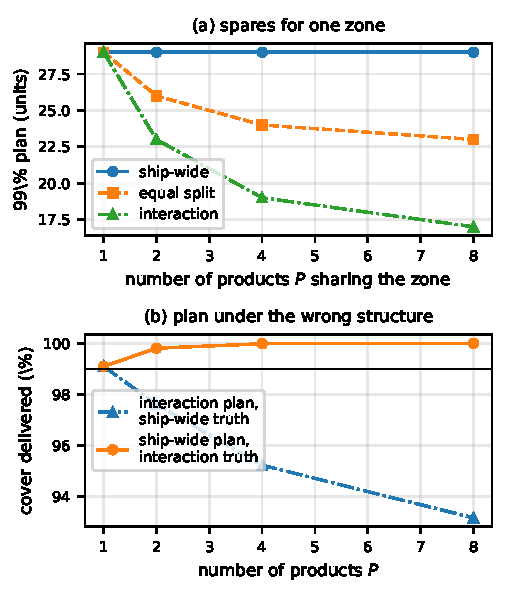
\includegraphics[width=\columnwidth]{figures/fig2_multiproduct.pdf}
\caption{Aggregate criterion~\eqref{eq:agg}, valid for interchangeable
references (\textsc{analytical}; the expected count \mpMean{} and the total
spread $\sigma=\mpSigma$ are assumed values). (top) The 99\,\% plan against the
number of references sharing the zone, under the two allocations of that spread
and an equal split. (bottom) Cover delivered when the plan is built under the
wrong allocation.}
\label{fig:multi}
\end{figure}

\begin{table}[!t]
\caption{Joint criterion~\eqref{eq:joint} against the aggregate
criterion~\eqref{eq:agg} at the 99\,\% level (\textsc{analytical}; expected
\mpMean{} failures over the zone and $\sigma=\mpSigma$ are assumed values).
$s_{\mathrm{marg}}$ is each reference's own marginal quantile and
$\gamma_{\mathrm{marg}}$ the joint cover it delivers; $s_{\mathrm{joint}}$ is the
smallest common per-reference stock meeting~\eqref{eq:joint}. The last two
columns compare total units under the two criteria: risk pools only when the
references are interchangeable}
\label{tab:stock}
\centering
\footnotesize
\setlength{\tabcolsep}{3.5pt}
\begin{tabular}{@{}clccccc@{}}
\toprule
& & \multicolumn{2}{c}{per-reference quantile} &
\multicolumn{2}{c}{joint~\eqref{eq:joint}} & agg.~\eqref{eq:agg} \\
\cmidrule(lr){3-4}\cmidrule(lr){5-6}\cmidrule(lr){7-7}
$P$ & structure & $s_{\mathrm{marg}}$ & $\gamma_{\mathrm{marg}}$ &
$s_{\mathrm{joint}}$ & total & total \\
\midrule
\tabinput{tables/tab_stock.tex}
\bottomrule
\end{tabular}
\end{table}

\subsection{Consequences}
Two conclusions for practice follow. The criterion must be fixed before the plan
is computed, since the two answers differ by a factor of order $P$ and respond to
the dependence structure with opposite signs: a fleet holding non-interchangeable
references uses~\eqref{eq:joint}, and the aggregate figure applies only to
interchangeable stock. Neither criterion should then be approached by adding
per-reference quantiles, since evaluating~\eqref{eq:conv}
and~\eqref{eq:jointexact}, or drawing from the fitted model, costs little.

The allocation between $\tau$ and $\omega$, however, is an empirical quantity that
no data in this paper determine, so a single data-holder $\sigma$ is not
sufficient to size a multi-reference plan under either criterion and none is
reported. While the ordering is unresolved, the defensible practice is to compute
the plan under both extremes and adopt the more conservative figure for the
criterion in force.


\section{Federated Estimation}
\label{sec:fed}
The constraint that motivates the model is that unit-level records are not
pooled. An estimator respecting it follows, together with what it does not
deliver.

\subsection{Local and Global Coordinates}
There are $S$ data holders and one coordinator: the ships of one operator
reporting to it, or the operators of a consortium reporting to a neutral
coordinator. Holder $s$ keeps its own cells $\mathcal C_s$, and every cell
belongs to exactly one holder.

The separation that makes the protocol possible is that both data-holding
terms of~\eqref{eq:structure} are local. The ship effect $u_s$ appears only in
the cells of ship $s$; so does each interaction effect $w_{sp}$, since it is
indexed by that ship and one of its $P_s$ references. Collect them in the local
latent vector
\begin{align}
\mathbf v_s&=(u_s,w_{s1},\dots,w_{sP_s})^{\top}\in\mathbb R^{1+P_s},
\label{eq:local}\\
\mathbf D_s&=\mathrm{diag}\big(\tau^{-2},\omega^{-2}\mathbf I_{P_s}\big),
\label{eq:localb}
\end{align}
with $\mathbf D_s$ the prior precision. The \emph{global} coordinates
$\boldsymbol\gamma$ are the shared ones: the coefficients $\boldsymbol\beta$, the
product and manufacturer effects, and any level above the holder. Holder $s$
touches only the $m_s$ global coordinates that appear in its own cells.

\subsection{Protocol}
For fixed variance parameters, let
\begin{equation}
\ell_s(\boldsymbol\gamma,\mathbf v_s)=\sum_{c\in\mathcal C_s}\log p(y_c\mid\cdot)
-\tfrac12\mathbf v_s^{\top}\mathbf D_s\mathbf v_s .
\end{equation}
At a proposed $\boldsymbol\gamma$ each holder solves for
$\hat{\mathbf v}_s(\boldsymbol\gamma)$ locally by a Newton iteration in
$1+P_s$ dimensions and returns
\begin{equation}
\Big(\ell_s,\ \nabla_{\gamma}\ell_s,\
\mathbf S_s=\mathbf H_{\gamma\gamma}^{(s)}-\mathbf H_{\gamma v}^{(s)}
\big(\mathbf H_{vv}^{(s)}\big)^{-1}\mathbf H_{v\gamma}^{(s)},\
\log\det\mathbf H_{vv}^{(s)}\Big),
\label{eq:message}
\end{equation}
evaluated at $(\boldsymbol\gamma,\hat{\mathbf v}_s)$, where $\mathbf H$ is the
negative Hessian and $\mathbf H_{vv}^{(s)}$ is the $(1+P_s)\times(1+P_s)$ local
block. The coordinator sums the messages, adds the prior precision $\mathbf P$ of
the global random effects, takes a damped Newton step in $\boldsymbol\gamma$ and
repeats; the resulting Laplace value
\begin{equation}
\sum_s\ell_s-\tfrac12\boldsymbol\gamma^{\top}\mathbf P\boldsymbol\gamma
-\tfrac12\Big[\sum_s\log\det\mathbf H_{vv}^{(s)}
+\log\det\big(\textstyle\sum_s\mathbf S_s+\mathbf P\big)\Big]
\label{eq:laplace}
\end{equation}
feeds an outer quasi-Newton search over the variance parameters
$(\tau,\omega,\phi,\dots)$.

The construction is exact rather than approximate because the joint negative
Hessian over $(\boldsymbol\gamma,\mathbf v_1,\dots,\mathbf v_S)$ is
block-arrowhead: $\mathbf v_s$ couples with $\boldsymbol\gamma$ only, and only
through the cells of holder $s$, so the blocks $\mathbf v_s$ and
$\mathbf v_{s'}$ are never coupled for $s\ne s'$. Eliminating each
$\mathbf v_s$ by its Schur complement gives
\begin{equation}
\det\mathbf H=\prod_s\det\mathbf H_{vv}^{(s)}\cdot
\det\Big(\textstyle\sum_s\mathbf S_s+\mathbf P\Big),
\end{equation}
and by the envelope theorem the step built from the messages is the Newton step
of the profiled joint objective. The iteration therefore reaches the same joint
mode as a centralised fit, and~\eqref{eq:laplace} equals the centralised Laplace
value up to the stopping tolerance. This is an instance of the federated
mixed-model literature~\cite{li2022fedglmm,luo2022dpql}, specialised so that the
whole local block, including every ship--product interaction, is eliminated
locally and never transmitted.

Two consequences of carrying the full local block follow. The local cost
rises from a scalar solve to a factorisation of order $(1+P_s)^3$, which is
negligible for the tens of references a zone carries. The transmitted quantities
are unchanged in dimension: only $\mathbf S_s$, of size $m_s\times m_s$ in the
global coordinates, and the scalar $\log\det\mathbf H_{vv}^{(s)}$ leave the
holder, so the interaction effects raise neither the message size nor what the
coordinator observes.

Holders of very different size enter unchanged. A ship that records no failure of
a product in a mission still returns a well-defined message, because its exposure
alone informs the rate and its own effect is shrunk towards zero, which is the
normal case on board and the reason such populations must not be dropped
(Section~\ref{sec:mechanisms}).

\subsection{Communication Cost}
A message~\eqref{eq:message} carries $2+m_s+m_s(m_s+1)/2$ numbers, so the cost per
round is quadratic in the global coordinates a holder touches and linear in the
number of holders, multiplied by the number of coordinator rounds. For the
cell-aggregated counts of this model, however, a single exchange of each
holder's cell table is also lossless for the
likelihood~\cite{luo2022dlmm,tong2025cola} and is cheaper whenever the cells per
holder are few, as for one product class on one ship. The iterative protocol is
therefore justified not by communication volume but by the cases in which a holder
will not release even the cell table, or in which covariates are continuous rather
than banded, so that no finite sufficient aggregate exists.

\subsection{Disclosure Properties}
The protocol establishes one property: \emph{no unit-level record leaves its
holder, and no holder's own effect is transmitted}. This is a statement about
data flow and not a confidentiality guarantee, and none is claimed here.

The messages are functions of the holder's cell aggregates
$\{(y_c,H_c,\mathbf x_c)\}_{c\in\mathcal C_s}$. An honest-but-curious
coordinator selects the parameter values at which those functions are evaluated
and receives many evaluations, and may therefore reconstruct the aggregates or
features of them. Sufficiency of an aggregate for estimation is not a bound on
what an adversary can infer. In addition, the set of global
coordinates a holder touches reveals which products it operates, which may be
commercially sensitive, and a minimum cell size limits what a single aggregate
describes without providing a formal guarantee. A deployment that
requires confidentiality must add secure aggregation or a differential-privacy
mechanism, and must then re-examine calibration, since noise added for privacy
enters the predictive distribution and therefore the plan.


\section{Identifiability and Campaign Design}
\label{sec:design}
Sections~\ref{sec:cover} and~\ref{sec:multi} show that a multi-reference plan
depends on how the latent spread is divided between a ship-wide term $\tau$ and
a ship--product term $\omega$. Whether a fleet's records could estimate that
division, and what a plan built from them delivers, can be answered by
simulation before any record is collected. Every number in this section is
simulated under assumed parameters.

\subsection{Design of the Study}
For ship $s$, reference $p$ and mission $t$ the generating model is
\begin{equation}
y_{spt}\sim\mathrm{Poisson}\!\left(m\,a_p\exp\{u_s+w_{sp}+e_{spt}
-\tfrac12(\tau^2+\omega^2+\varepsilon^2)\}\right),
\label{eq:sim}
\end{equation}
with $u_s\sim\mathcal N(0,\tau^2)$, $w_{sp}\sim\mathcal N(0,\omega^2)$ and a
mission term $e_{spt}\sim\mathcal N(0,\varepsilon^2)$, so that each cell expects
$m\,a_p$ failures. The reference weights $a_p$ are equal or proportional to
$1:2:4:8$. Five allocations are studied: ship-wide only $(\tau,\omega)=(0.6,0)$,
interaction only $(0,0.6)$, equal splits $(0.42,0.42)$ and $(0.3,0.3)$, and none
$(0,0)$. A full factorial in the number of ships $S\in\{5,10,20,40,80\}$ and
missions per ship $M\in\{1,2,4,8\}$, with $P=4$, $m=1$ and $\varepsilon=0.3$, is
completed by one-factor variations of $m\in\{0.1,0.3,3\}$, $P\in\{2,8\}$,
$\varepsilon\in\{0,0.6\}$ and unequal weights: \dsCells{} cells of \dsReps{}
campaigns each, \dsCampaigns{} in all.

Every campaign is fitted three times with the estimator of
Section~\ref{sec:model} (both terms, ship term only, interaction term only,
reference as a fixed effect), which gives the estimates and the likelihood-ratio
statistic for each term. Because a variance at zero lies on the boundary of the
parameter space, the statistic is referred to an equal mixture of
$\chi^2_0$ and $\chi^2_1$~\cite{self1987,stram1994}. In 15 cells the first 300
campaigns also receive profile-likelihood intervals for $\tau$ and $\omega$.
A 99\,\% plan for one mission of an unseen ship is then built from each fit in
four ways: \emph{plug-in}, from draws of the latent terms at the estimated
parameters; \emph{predictive}, adding draws of the coefficients from their
approximate posterior; \emph{conservative}, the larger of the plug-in plans with
the estimated total spread put wholly on $\tau$ and wholly on $\omega$; and
\emph{Poisson}, each reference at its own Poisson quantile. The cover each plan
delivers is computed exactly under the true model~\eqref{eq:sim} by
Proposition~\ref{prop:multi}, with the mission term folded into the reference
term. Monte Carlo standard errors follow~\cite{morris2019}: \dsMcseRej{}
percentage points for a rejection rate near 5\,\%.

No campaign failed to fit. The conditioning is specific: the latent effects are
Gaussian, $\varepsilon$ is fixed within a cell and there are no common-cause
events, reference changes or reporting errors. Section~\ref{sec:fleet} relaxes
those assumptions.

\subsection{Testing and Estimating the Allocation}
The boundary test holds its size. Across the cells where a component is zero
the rejection rate at the 5\,\% level has median \dsTypeOneMed\,\% and maximum
\dsTypeOneMax\,\%, conservative as the mixture theory predicts. A spurious
component is therefore no more frequent than the test allows, provided it is
tested and not judged from whether a point estimate leaves the boundary, which
happens about half the time under the null whatever the campaign size.

Table~\ref{tab:power} gives the power under the equal split $(0.42,0.42)$.
With one mission per ship the interaction term is never detected, at any
number of ships: it varies at the same level as the mission term and cannot be
told apart from it, and when the truth is interaction only the larger component
is identified correctly in only \dsOrderOneLo--\dsOrderOneHi\,\% of campaigns.
Repeated missions are what identifies it. With four missions, the interaction
is detected in \dsPowOmTenFour\,\% of ten-ship campaigns and
\dsPowOmTwentyFour\,\% of twenty-ship ones, and with eight missions and forty
ships in \dsPowOmFortyEight\,\%. With at least four missions and ten ships the
larger component is identified in at least \dsOrderFour\,\% of campaigns. The
profile intervals cover the true values in \dsCiLo--\dsCiHi\,\% of the
\dsCiReps{} campaigns per cell against a nominal 95\,\%.

\begin{table}[!t]
\caption{Power of the boundary likelihood-ratio test at 5\,\% when both
components are present, $(\tau,\omega)=(0.42,0.42)$, in percent
(\textsc{simulation}, \dsReps{} campaigns per cell, $P=4$, $m=1$)}
\label{tab:power}
\centering
\footnotesize
\setlength{\tabcolsep}{4.5pt}
\begin{tabular}{@{}ccccccccc@{}}
\toprule
& \multicolumn{4}{c}{ship-wide $\tau$, missions $M$} &
\multicolumn{4}{c}{interaction $\omega$, missions $M$} \\
\cmidrule(lr){2-5}\cmidrule(lr){6-9}
$S$ & 1 & 2 & 4 & 8 & 1 & 2 & 4 & 8 \\
\midrule
\tabinput{tables/tab_power.tex}
\bottomrule
\end{tabular}
\end{table}

\subsection{Cover of Plans for an Unseen Ship}
Table~\ref{tab:campaign} reports the joint cover delivered by each plan,
averaged over the five allocations. The predictive plan reaches its target from
ten ships on (\dsPredCoverTen\,\%), and in no cell with at least ten ships and
two missions does its mean fall below \dsPredMin\,\%. The plug-in plan, which
ignores the uncertainty of the coefficients, falls short when the campaign is
small (\dsPlugCoverFive\,\% with five ships). The conservative plan behaves
like the plug-in one at slightly higher cost. The Poisson plan delivers
\dsPoisLo--\dsPoisHi\,\% across allocations, \dsPoisMThree\,\% when each cell
expects three failures and \dsPoisPEight\,\% with eight references, since its
shortfall grows with the count and with the number of references that must
all be covered.

The price of a small campaign shows in the stock rather than in the cover.
With five ships the predictive plan has a median of \dsUnitsFiveMed{} units,
close to the \dsUnitsOracle{} of the plan that knows the parameters, but a mean
of \dsUnitsFiveMean: in a minority of campaigns the coefficients are so poorly
determined that the plan becomes very large. That is the correct response of a
predictive distribution to little evidence, and it is what a fleet with five
ships should expect to pay.

\begin{table}[!t]
\caption{Mean joint cover of a 99\,\% plan for a four-reference zone of an
unseen ship, in percent, averaged over five allocations, with the mean tenth
percentile of the predictive plan and median units of the predictive and
oracle plans (\textsc{simulation}; $M=4$)}
\label{tab:campaign}
\centering
\footnotesize
\setlength{\tabcolsep}{3.2pt}
\begin{tabular}{@{}cccccccc@{}}
\toprule
$S$ & plug-in & predictive & conservative & Poisson & pred. p10 &
\multicolumn{2}{c}{units (pred./oracle)} \\
\midrule
\tabinput{tables/tab_campaign_cover.tex}
\bottomrule
\end{tabular}
\end{table}

\subsection{Implications for a First Campaign}
Within the configurations examined, a campaign should follow several references
on the same ships over repeated missions; breadth in ships does not substitute
for repetition, and a cross-sectional snapshot cannot separate the two terms at
all. Ten ships over four missions is the smallest configuration in this grid
that orders the components reliably, and twenty to forty ships detect the
interaction with high probability. Plans should be computed from the full
predictive distribution, which keeps its cover in small campaigns at the cost
of stock, and the components should be reported with their intervals and
tests.


\section{A Simulated Passenger Fleet}
\label{sec:fleet}
Every number in this section is simulated; no number describes a real fleet.

\subsection{Fleet, Parameters and Scenarios}
The fleet has \flShips{} ships in five classes, from an expedition ship of 92
cabins to one of about 2\,750 and a cruise ferry, with the seven references of
Section~\ref{sec:ship}, each made by two makers, one per class. Parameters are
of four kinds; none is an estimate transferred from another source.
\emph{Published}: cabins per class from shipyard fact
sheets~\cite{fincantieri_laperouse,oasis_class}; datasheet predictions at
reference conditions, not observed values, of MTBF 2.19 to 9.09 million hours
for the drivers and supplies (Telcordia SR-332; e.g.~\cite{meanwell_lpv60}) and MTTF
0.54 and 0.56 million hours for the drives (IEC 62380)~\cite{schneider_atv212},
whose inverses serve as nominal \emph{datasheet rates} under a constant-rate
assumption; climate normals; and the mean cruise of 7.0
days~\cite{clia2025}. \emph{Assumed within a published range}: an activation
energy of 0.5\,eV, within MIL-HDBK-217F's values for silicon
microcircuits~\cite{milhdbk217f}. \emph{Assumed, motivated by published
values}: a field factor of 3, below the 5 to 12 by which the handbook raises
naval sheltered over ground benign environments by part class and near a pooled
conversion of 3.3~\cite{jeong2011}. \emph{Assumed}: a bad-lot factor
of 2.5, for which a street-lighting programme whose LED fixtures failed in
their drivers~\cite{halifax2019} shows only that defective driver lots occur;
drivers per cabin
and public area, costs, a Weibull age shape of 1.3, lognormal ship,
ship--reference, maker and cell terms of standard deviation 0.3, 0.3, 0.3 and
0.15, the distribution of cruise lengths (3 to 14 nights, 1 to 2 for the
ferry), and every event and recording parameter. Activation energy and age
shape reach the plans only through temperature and age slopes fitted to the
record. Planned powered hours follow from booked occupancy and climate
normals, failures from realised ones. Of two simulated years, the
first eighteen months of all ships but one per class are fitted and the last
six predicted, at known and at held-out new ships: about \fdMissions{}
ship-missions per fleet.

\emph{Clean} meets the model. \emph{Baseline} adds ship-wide supply events at
0.2 per ship-year, each failing 0.05\,\% of every population; a bad lot
multiplying one reference's rate by 2.5 on half the ships of a class; refits
renewing cabin units; and 10\,\% of preventive replacements recorded as
failures. Other scenarios vary one assumption: truncated Student-$t_3$ latent effects;
25\,\% misrecorded replacements; half the fleet observed for one year;
datasheets that are right (field factor 1); and events at 0.5 per ship-year
failing 0.1\,\%, and at 2 failing 0.05\,\% or 0.2\,\%. The generator draws one
event state per ship-mission, with probability $1-e^{-rH/365}$ for rate $r$
and $H$ nights, and an event adds $\mathrm{Binomial}(N,a)$ failures to every
population; it never places two events in one mission. No public source gives
$r$ or $a$ for events that damage electronics; whole-ship losses of electrical
power on passenger ships, about 0.005 per ship-year from EMSA's 2024 indicator
of 247 occurrences per 1\,000 ship-years times their 2.1\,\% share (our
derivation)~\cite{emsa2025} and 24 in the UK from 2020 to May 2026, without
exposure~\cite{maib_portal}, are context only.

\subsection{Plans and Comparators}
Every plan targets a nominal 99\,\% joint cover for one ship-mission from
pre-sailing information, minimising units under the law used to plan it, and
is scored on realised failures of missions not used to fit or select it; the
term \emph{certified optimum} is reserved for vectors whose search finished.
The \emph{datasheet} benchmark plans for independent Poisson
counts at datasheet rate times planned hours; the \emph{scaled} plan
multiplies those rates by one fleet-wide factor fitted to the record; the
\emph{pooled negative binomial} has covariates and maker but no ship terms.
The \emph{hierarchical} plan uses \brDraws{} predictive draws of the model with
maker, ship and ship--reference terms, and the \emph{fixed-marginal predictive
comparator} the same draws with each reference column permuted independently,
which keeps every empirical marginal and breaks the dependence; it is not the
$f=0$ law of Proposition~\ref{prop:mono} and carries no guarantee.

For draw-based plans the planning law is the empirical law of the draws, and
minimisation is by iterative deepening on the units above the marginal
quantiles. It was certified for all but \fdNotCertJP{}
joint or fixed-marginal and \fdNotCertEv{} incident plans of about
\fdPlansPerType{} per plan type (at least \fdCert\,\% in every group), all
with severe events; these keep the best vector found, feasible under the draws
and at most \fdNotCertGap{} units above a lower bound. With a new seed or
24\,000 draws, only \fdStabSameSeed\,\% and \fdStabSameBig\,\% of vectors on
\fdStabFleets{} fleets were unchanged, yet mean cover stayed at least
\fdStabFresh\,\%: performance is stable where the vector is not.

\begin{table*}[!t]
\caption{Simulated fleet: cover $J$ (\%) and units u per mission of
unit-minimal plans for a nominal 99\,\%; hierarchical (joint) minus fixed-marginal plan from the
same draws, in points ($\Delta J$, 95\,\% interval resampling fleets) and
units ($\Delta$u); italics: $J<99$\,\%, star: interval below 99\,\%
(\textsc{simulation}; \fdFleets{} fleets per scenario)}
\label{tab:fleet}
\centering
\footnotesize
\setlength{\tabcolsep}{1.6pt}
\begin{tabular}{@{}lcccccrlrcrlr@{}}
\toprule
& \multicolumn{8}{c}{known ships} & \multicolumn{4}{c}{new ships} \\
\cmidrule(lr){2-9}\cmidrule(l){10-13}
& datash. & scaled & pooled & hier. & fixed & \multicolumn{2}{c}{$\Delta J$} &
$\Delta$u & hier. & \multicolumn{2}{c}{$\Delta J$} & $\Delta$u \\
Scenario & $J$ & $J$/u & $J$/u & $J$/u & $J$/u & & & & $J$/u & & & \\
\midrule
\tabinput{tables/tab_fleet5.tex}
\bottomrule
\end{tabular}
\end{table*}

\subsection{Rates, Marginals and Dependence}
Table~\ref{tab:fleet} separates three contributions; ranges are over the
scenarios without frequent events. \emph{Learning field rates}: the datasheet
benchmark covers \fdMtbfLo--\fdMtbfHi\,\% of missions at known ships when the
field rate exceeds the datasheet rate, as the design builds in, and
\fdMtbfRight\,\% when datasheets are right; one fleet-wide factor raises this
to \fdScaledLo--\fdScaledHi\,\%. \emph{Estimating each ship's marginal laws}: the pooled,
hierarchical and fixed-marginal plans cover \fdFitKLo--\fdFitKHi\,\% at known
ships and \fdFitNLo--\fdFitNHi\,\% at new ones; in the baseline the
hierarchical plan differs from the pooled negative binomial by \fdJpCov{}
points (\fdJpCovLo{} to \fdJpCovHi) and \fdJpUn{} units (\fdJpUnLo{} to
\fdJpUnHi) per mission at known ships, and by \fdJpNewCov{} points and
\fdJpNewUn{} units at new ones. Joint cover still differs from marginal cover:
per-reference 99\,\% quantiles taken separately cover only
\fdMargLo--\fdMargHi\,\% jointly. \emph{Modelling dependence}: against the
fixed-marginal comparator the hierarchical plan changed cover by \fdDcKLo{} to
\fdDcKHi{} points at known ships and \fdDcNLo{} to \fdDcNHi{} at new ones,
every interval within \fdDcCiKLo{} and \fdDcCiNHi{} points, and saved at most
\fdAbsDuMax{} units per mission, systematically only at new ships. The
permutation left up to \fdResid{} points of residual dependence, the order of
the contrast.

\begin{table}[!t]
\caption{Bridge, large ship: unit-minimal 99\,\% plan with dependence minus
plan under independence, exact and from draws (mean $\pm$ 95\,\% half-width,
\brSeeds{} seeds), scored exactly at the true $f$ (\textsc{exact and
simulation}; $H$
days, $\Lambda$ expected failures, u units at $f=0$)}
\label{tab:bridge}
\centering
\footnotesize
\setlength{\tabcolsep}{2.2pt}
\begin{tabular}{@{}lrrrrrrr@{}}
\toprule
& & & \multicolumn{2}{c}{exact $\Delta$u} & \multicolumn{3}{c}{draws} \\
\cmidrule(lr){4-5}\cmidrule(l){6-8}
$H$ & $\Lambda$ & u & $f{=}0.5$ & $f{=}1$ & $\Delta$u, 0.5 & $\Delta$u, $f{=}1$ &
$\Delta J$, $f{=}1$ \\
\midrule
\tabinput{tables/tab_bridge.tex}
\bottomrule
\end{tabular}
\end{table}

Table~\ref{tab:bridge} links that contrast to the proposition. For the large ship each horizon fixes the marginal
laws, with means proportional to $H$ and a latent multiplier persisting until
resupply, while $f$ varies; plans from \brDraws{} draws of the true law are
set against plans from the same draws permuted. At $f=0$ the draw contrast is Monte Carlo
error, within $\pm$\brNoiseU{} units and $\pm$\brNoiseJ{} points. At the
fleet's spreads, $\sigma=0.42$, and a weekly horizon the exact plans coincide
and the draw contrast is \brFleetDu{} units, as in Table~\ref{tab:fleet}.
Dependence pays when horizon and ship-wide spread grow together: at
$\sigma=0.6$, $f=1$ and 56 days the dependent optimum needs \brBigDep{} units
against \brBigInd, \brBigSave{} or \brBigUnitPct\,\% fewer. These plans
minimise units, as in the fleet; Table~\ref{tab:ship} minimises relative cost.
Plans chosen on draws are nominally 99\,\% and meet it on their draws, but
their mean exact cover was \brJLo--\brJHi\,\%, the error of selecting on a
sample.

\subsection{Supply Events}
Table~\ref{tab:ev} adds to the hierarchical draws an explicit incident term of
the generator's form, one event state per mission adding
$\mathrm{Binomial}(N_p,a)$ failures to every reference, and replans to 99\,\%
joint cover per mission under that law. With the generating $r$ and $a$ it is
an idealised reference; both are also misstated by factors of 0.5 and 2.

\begin{table}[!t]
\caption{Plans with an explicit incident term, known ships: cover (\%), mean
units, units above the plan without the term, units short per event mission
(\textsc{simulation}; \fdFleets{} fleets)}
\label{tab:ev}
\centering
\footnotesize
\setlength{\tabcolsep}{2.4pt}
\begin{tabular}{@{}lcccccc@{}}
\toprule
& \multicolumn{3}{c}{$J$ (\%)} & & & short \\
\cmidrule(lr){2-4}
Plan & all & event & no event & units & extra & /event \\
\midrule
\tabinput{tables/tab_ev.tex}
\bottomrule
\end{tabular}
\end{table}

Without an event term the hierarchical plan covered \fdEvFreqOmitEv\,\%
(\fdEvFreqOmitEvLo--\fdEvFreqOmitEvHi) of event missions at two events a year
failing 0.05\,\%, and \fdEvSevOmitEv\,\% when each fails 0.2\,\%; the
idealised plan raised these to \fdEvFreqKnownEv{} and \fdEvSevKnownEv\,\% and
overall cover from \fdEvFreqOmitAll{} to \fdEvFreqKnownAll{} and from
\fdEvSevOmitAll{} to \fdEvSevKnownAll\,\%, for \fdEvFreqExtra{} and
\fdEvSevExtra\,\% more units. The model of incidents buys this cover and its
parameters size the stock: halving the stated size lost half or more of the
gain on event missions, halving the rate less, and doubling either bought
further cover with stock. In the baseline (\fdEvBaseN{} event missions of
\fdEvBaseAll) it left event-mission cover unchanged (\fdEvBaseOmitEv{} and
\fdEvBaseKnownEv\,\%): events are rarer than the 1\,\% the target allows.


\section{A Real Fleet: LED Street Lighting}
\label{sec:lighting}
A public street-lighting network has the structure of the provisioning problem
on ships: LED drivers of several product families, installed in populations of
known size, divided among maintenance units that each hold their own spares, and
exposed to events that put a whole street out at once. This section applies the
method to such a network; every number in it is measured, from public records.

\subsection{Data}
The Department for Infrastructure of Northern Ireland publishes, under the Open
Government Licence, every fault report on its street lighting since 2020 and an
inventory of its about 300\,000 lighting points with the lantern type of each~\cite{dfi_lighting}.
An operational area plays the part of a ship, a lantern family the part of a
product reference and a month the part of a mission. Eight LED families are
distinguished, seven named product lines and a residual group, the smallest
with about 2\,000 points on the streets used. Fault reports carry the street but not the lantern, so only
streets equipped with a single family are used, where the attribution is exact;
they hold about 166\,000 LED points. A report of a single light out is taken as
demand for a lantern spare. Reports closed as cable or supply faults, or as no
fault found, are excluded, and a report within seven days of the previous one on
the same street is counted as the same repair, which removes about a third of
the reports. Exposure is the installed count times the dusk-to-dawn hours of
the month at the network's latitude, and the calendar month enters as a fixed
effect for seasonal reporting.

The inventory is a snapshot, and older lanterns were still being replaced by
LED during the period. The models are therefore fitted on April 2023 to
March 2025 with the snapshot of April 2025, a total of \niTrainFail{} failures
over \niAreas{} areas and \niFamilies{} families. Two tests are made: a split
within that period, fitting on its first year (\niWithinTrain{} failures) and
predicting the second (\niWithinTest{} failures, \niWithinMonths{} area-months),
and a forward test on April to October 2026 with the November 2026 snapshot
(\niForwardTest{} failures, \niForwardMonths{} area-months). Each test is run
once with all areas in the fit and once leaving each area out in turn, as a
holder never seen before.

\subsection{The Allocation, Measured}
Fitted with an area term, an area--family interaction and an area--month term,
the network gives an area-wide standard deviation of \niSigArea{} (profile
interval \niCiArea, boundary test $p=\niPArea$), an interaction of
\niSigInter{} (\niCiInter, $p\niPInter$) and a month term of \niSigMonth{}
(\niCiMonth, $p=\niPMonth$). Family rate ratios range from \niFamLo{} to
\niFamHi{} relative to the reference family. On this network the heterogeneity
between holders is almost entirely of the interaction kind: an area is not
worse for every family, but particular families do markedly better or worse in
particular areas. Under the aggregate criterion this is the allocation for which
risk pools best, and under the joint criterion the one that is hardest to
cover (Section~\ref{sec:multi}). The shared month term, the analogue of a
ship-wide event, is small but detectable.

\subsection{Plans Tested Out of Sample}
Table~\ref{tab:ni} gives the joint cover of a 99\,\% plan over the families an
area holds. In the within-period test with known areas, the Poisson plan covers
\niPoissonWithinKnownCover\,\% of area-months and the empirical-Bayes plan
\niEbGammaWithinKnownCover\,\%. The hierarchical predictive plan covers
\niHierPredWithinKnownCover\,\% with \niHierPredWithinKnownUnits{} units, against
\niPoissonWithinKnownUnits{} for Poisson and \niNbPooledWithinKnownUnits{} for
the pooled negative binomial, which reaches \niNbPooledWithinKnownCover\,\%.
Knowing which families run high in which area is what lets the hierarchical
plan reach the target without the pooled model's uniform margin.

For an area left out of the fit the picture changes. The interaction of an
unseen area is unknown, and with a standard deviation of \niSigInter{} the
hierarchical plan has to cover it, at \niHierPredWithinNewUnits{} units. The
pooled negative binomial, which spreads the same heterogeneity over all cells,
covers \niNbPooledWithinNewCover\,\% with \niNbPooledWithinNewUnits{} units,
while Poisson and empirical Bayes fall to \niPoissonWithinNewCover{} and
\niEbGammaWithinNewCover\,\%. For a new holder the large interaction makes the
hierarchical plan safe but expensive, and its history, once available, is
worth most of that stock.

The forward test fell in a quieter year: failure rates in April to October 2026
were below those of the fitting period, and every plan covered every
area-month, Poisson with \niPoissonForwardKnownUnits{} units and the
hierarchical predictive plan with \niHierPredForwardKnownUnits. It confirms that
the plans are not exceeded a year ahead but cannot separate the methods; a
fleet should expect drifts of this kind and refit as records accumulate.

\begin{table}[!t]
\caption{Northern Ireland street lighting: joint cover (\%) of a 99\,\% plan
over an area's families, mean units per area-month and mean log score per
family-month
(\textsc{measured}; new areas are left out of the fit in turn)}
\label{tab:ni}
\centering
\footnotesize
\setlength{\tabcolsep}{2.6pt}
\begin{tabular}{@{}lccccccc@{}}
\toprule
& \multicolumn{5}{c}{within-period test} & \multicolumn{2}{c}{forward test} \\
\cmidrule(lr){2-6}\cmidrule(lr){7-8}
& \multicolumn{3}{c}{known areas} & \multicolumn{2}{c}{new area} &
\multicolumn{2}{c}{known areas} \\
\cmidrule(lr){2-4}\cmidrule(lr){5-6}\cmidrule(lr){7-8}
Plan & cover & units & log sc. & cover & units & cover & units \\
\midrule
\tabinput{tables/tab_ni.tex}
\bottomrule
\end{tabular}
\end{table}


\section{Limitations and Requirements for Validation}
\label{sec:limits}
\subsection{Scope of the Results}
Three classes of statement are supported. The analytical class:
Propositions~\ref{prop:exact} and~\ref{prop:multi} are exact under their stated
assumptions, and the figures accompanying Proposition~\ref{prop:approx} are maxima
observed on the stated grid, properties of the idealised mixture rather than of any
fleet. The simulated class: everything in Section~\ref{sec:design} is generated
under~\eqref{eq:sim} with assumed parameters. The measured class: only the capacitor
figures of Section~\ref{sec:evidence}. A manifest accompanying the code gives every
reported value's script, result file and provenance tag; no tag denotes a shipboard
measurement, because there is none.

\subsection{Limitations}
\subsubsection{No Shipboard Quantity}
No failure rate, temperature coefficient, variance
component, coverage or spares count for shipboard power electronics is reported,
because none could be estimated. The values $\sigma=\mpSigma$ and $\tau,\omega$
used in Sections~\ref{sec:multi} and~\ref{sec:design} illustrate the arithmetic
and must not be quoted as fleet characteristics.

\subsubsection{No Empirical Calibration}
No predictive interval has been checked against
observed shipboard failures, so the calibration of the predictive distribution
remains open and is the first thing a campaign should test.

\subsubsection{No Identified Dependence Structure}
The division of latent spread between
the ship-wide and interaction terms is not determined by any evidence here. Since
it changes a multi-reference plan materially under either criterion
(Section~\ref{sec:multi}) and is difficult to estimate
(Section~\ref{sec:design}), this limits any provisioning recommendation,
including the one developed here.

\subsubsection{Idealised Theory}
Propositions~\ref{prop:exact} and~\ref{prop:approx}
concern the mixed-Poisson case~\eqref{eq:mixture}, not the full model with its
cell dispersion, crossed effects and parameter uncertainty; the common-cause and
cascading mechanisms of Section~\ref{sec:mechanisms} are outside
Assumption~\ref{as:mix} altogether and act on the upper tail, where a
provisioning quantile lies. A plan computed under Assumption~\ref{as:mix} will
understate the stock required if such events occur at non-negligible rates.

\subsubsection{No Remaining-Life Estimate}
The model gives a failure count over a bounded
horizon; extending it to remaining life requires unit-level time-to-event records
and a survival or recurrent-event formulation~\cite{meeker2022} within the same
hierarchy. Finally, the federated protocol is not the cheaper option for
cell-aggregated counts and offers no confidentiality guarantee
(Section~\ref{sec:fed}).

\subsection{Requirements for Empirical Validation}
\label{sec:needed}
Six records are necessary. The first is an inventory of the installed population
by ship, zone, reference, manufacturer and installation date, maintained through
refits. The second is a set of event records in which every replacement is dated
and classified as functional failure or preventive by a rule fixed in advance,
with removals for refit, obsolescence and cannibalisation recorded separately;
where that classification is ambiguous the ambiguity must be quantified and the
analysis repeated under both readings. The third is exposure in powered
unit-hours per population and mission. The fourth is a set of covariates logged
over complete missions, so that the previous mission's summaries exist at the
moment of decision, since a covariate available only contemporaneously cannot
enter this decision however predictive it is. The fifth is repeated missions and
several references per ship, without which the two terms of~\eqref{eq:structure}
cannot be separated (Section~\ref{sec:design}). The sixth is a record of
common-cause events, together with teardown of a sample of removed units, so
that conditional independence and the limiting failure mode are tested rather
than assumed.

With such records the analysis developed here can be carried out on ships, and its
calibration, variance components and dependence structure become measurable. In
their absence those quantities cannot be estimated, and none is reported.


\section{Conclusion}
\label{sec:conclusion}
This paper has built the predictive distribution of a passenger ship's mission
failure count from a hierarchical model with crossed ship-wide and ship--product
terms, fitted from pooled or divided records, and has followed it through to the
spares a ship embarks.

For one population, the negative binomial matched to the moments of the mixture
is close to the exact plan, at most \spNbShort{} points short at the 99\,\%
level on the grid examined, and can be used where the exact computation is not
available. The Poisson plan and the variance-inflated margin should not be. For
a zone with several references, the plan is a vector whose cover depends on how
the heterogeneity divides between ship and product. Per-reference quantiles fall
short of a joint target, cost-minimal vectors save a median \rvSaveMed\,\% over
a common stock, and while the division is unknown a conservative plan keeps the
target at a premium in stock.

In the simulated passenger fleet the largest loss came from planning with
datasheet rates, which covered \flMtbfJointLo--\flMtbfJointHi\,\% of missions
against a 99\,\% target even as a joint plan. Joint plans fitted to the fleet's
own records covered \flStatLo--\flStatHi\,\% under supply events, bad lots,
heavy-tailed effects and misrecorded replacements, and from half the fleet over
one year. With the moderate heterogeneity assumed there, the hierarchy added
little to a pooled negative binomial on average, but it kept its stock in
proportion when one ship lay far in the tail, and the pooled model did not. On
the street-lighting network, where the
interaction between area and family was more than twice as large, the
hierarchical plans were the only ones to meet the target in the held-out year,
with fewer units than the pooled negative binomial in known areas and at a
high price for an area never seen.

What the model needs from a fleet's records is set out in
Section~\ref{sec:needed}: several references followed on the same ships over
repeated missions, ten ships or more, exposure in powered hours and a record of
common-cause events. Applying it to such records is the next step.


\section*{Acknowledgment}
The authors used Claude (Anthropic) to review the manuscript and the analysis
code and to suggest improvements to both. The authors checked every suggestion,
verified all code, results and text, and take full responsibility for the
content of this article.

\bibliographystyle{IEEEtran}
\bibliography{references}

\begin{IEEEbiographynophoto}{Paula Lamo}
(Senior Member, IEEE) received the bachelor's degree in naval engineering and
marine engineering from the University of Cantabria, Cantabria, Spain, in 2010;
the master's degrees in maritime engineering and teacher training from the
University of Cantabria, in 2011; the integrated master's degree in management of
environmental quality and occupational risk prevention and renewable energy, and
the master's degree in occupational risk prevention and industrial engineering
from University CEU San Pablo, Madrid, Spain, in 2012, 2013, and 2014,
respectively; and the Ph.D. degree in occupational risk prevention and industrial
engineering from the University of Cantabria, in 2019.

From 2019 to 2025, she was an Associate Professor with the Universidad
Internacional de La Rioja, Logro\~no, Spain. Since then, she has been an
Associate Professor with the Universidad de Cantabria, Santander, Spain. She is
also the President of the IEEE Power Electronics and Industrial Electronics
Spanish Chapter.
\end{IEEEbiographynophoto}

\begin{IEEEbiographynophoto}{Ricardo S. Alonso}
received the Ph.D. degree in computer engineering from the University of
Salamanca, Salamanca, Spain.

He is currently a Senior Lecturer with the Universidad Internacional de La Rioja
(UNIR), Logro\~{n}o, Spain, where he serves as Academic Director of two master's
programmes in artificial intelligence, and Director General of the AIR
Institute, Salamanca, Spain, a nationally recognised research and technology
centre specialised in artificial intelligence and computer science. He has
authored numerous contributions in JCR-indexed journals, international
conferences, and book chapters. He has coordinated and participated in
regional, national, and European R\&D projects, including Horizon Europe,
PRIMA, and CDTI initiatives, and coordinates the DIGIS3 European Digital
Innovation Hub. He previously co-founded NEBUSENS, a technology company devoted
to wireless sensor networks and real-time location systems. His research
interests include artificial intelligence, multi-agent systems, the Internet of
Things, wireless sensor networks, edge computing, and federated learning.

Dr. Alonso holds two six-year research periods recognised by the Spanish
National Commission for the Evaluation of Research Activity (CNEAI).
\end{IEEEbiographynophoto}

\end{document}
